\chapter{The Delta Scuti stars}
\label{deltascuti}
In this chapter we characterize describe the $\delta Sct$ stars more in detail, including the stars used in this work. 
\begin{figure}[htbp]
    \centering
    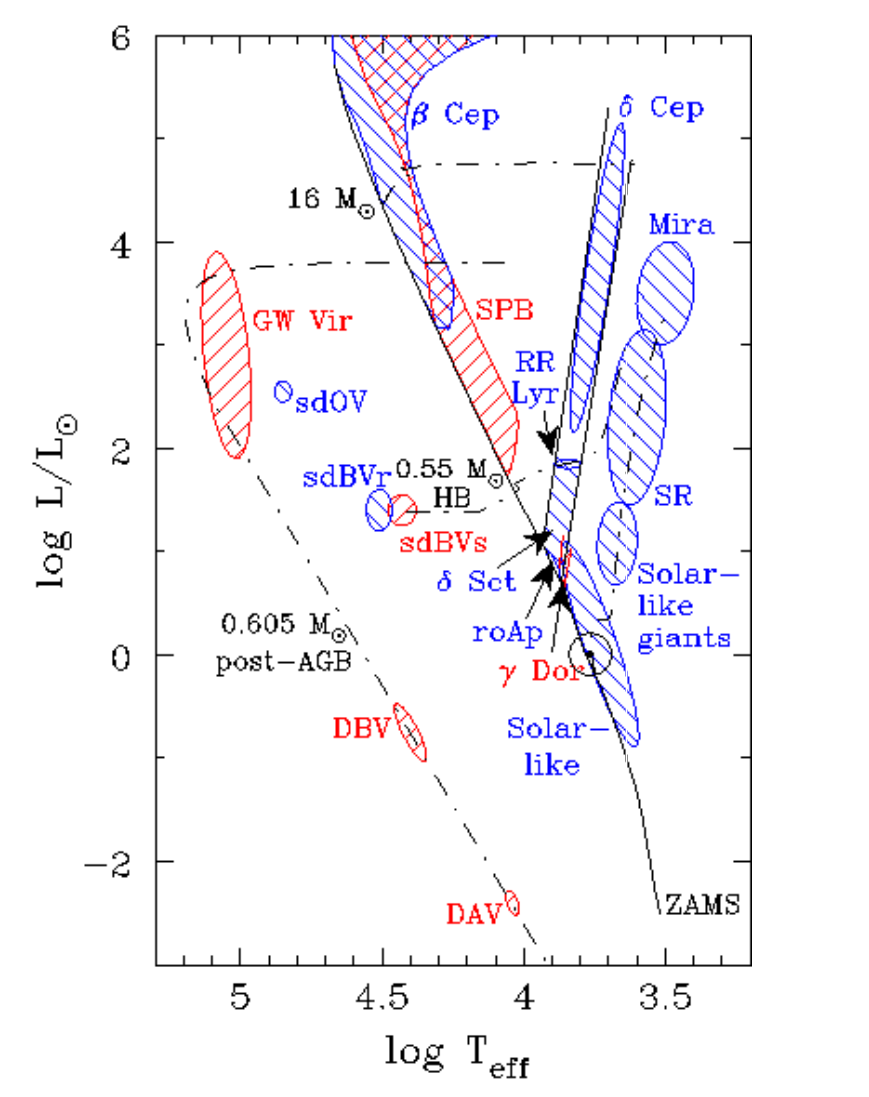
\includegraphics[width=0.9\textwidth]{hrpuls.png}
    \caption{Asteroseismic HR-diagram, showing the different classifications of pulsating stars. }
    \label{hrd}
\end{figure}

\section{The pulsation HR-diagram and the driving mechanisms}
As mentioned in the introduction, there are many different types of pulsating stars, situated over the entire Hertzsprung-Russel diagram (HR-diagram). \figref{hrd} illustrates the schematic overview of the various type in the \textit{asteroseismic HR-diagram}. Stars that have p-mode pulsations are marked in red, whereas g-mode pulsators are blue. They range in the HR-diagram for which the various types pulsate are called their \textit{instability strip}. Some stars can pulsate in both p and g-modes simultaneously. These types are called \textit{hybrids}, and can be found where the instability strips overlap. 

The type of oscillation a star pulsates with depends on the \textit{driving mechanism}. For the Sun and solar like-oscillators the primary driving mechanism is the stochastic driving. Acoustic energy from motion in convective cells in the outer convection zone can sufficiently cause a resonance at the star's natural frequencies, where a part of the energy becomes oscillation modes. A mode will be excited in a convection cell and damped when the cell turn over. But since there is a large number of convective cells it will be re-excited immidiately after at a different phase. So the excitation is random or \textit{stochastic}. 
For $\delta$ Sct stars, the driving mechanism is different. These are driven by a heat engine, which is a mechanism that transforms thermal energy in a star into mechanical energy of oscillations. When a star contracts the pressure and temperature increases, causing the opacity ($\kappa$) to increase in layers of H and He ionization. The radiative flux from the core is hence blocked and builds up underneath the layers of higher opacity. When the star reaches a thermodynamic equilibrium the additional stored energy in transformed into mechanical energy, causing the layers to move beyond the equilibrium; the star expands. But the ionization of the gas causes a reduction in opacity and radiation can flow through. The gas then cools down so much that it can no longer support the weight of the overlying layers, and the star then contracts recombining H and He. The cycle then repeats itself. 
The zones where the radiative flux becomes trapped are the layers of partial ionization. The first zone is where H and He are ionized around 14.000 K, close to the surface of the star. Second ionization zone is around 40.000 K where He II is partially ionized. Lastly, the innermost zone is where ionization of iron elements occur, at 200.000 K. For $\delta$ Sct stars the driving mechanism excites primarily in the He II ionization layer along with RR Lyrae and Cepheid stars. 

Yet another type of driving mechanism is the \textit{convective blocking} in Gamma Doradus ($\gamma$ Dor), DA and DB dwarfs. This mechanism is similar to the $\kappa$ mechanism, except the energy is stored in the outer convection zones. Such mechanism gives rise to g-modes oscillations rather than the p-modes from the $\kappa$ mechanism. 

Compared to the stochastic excitations in solar-like oscillators, the heat engine mechanism does not excite all modes to an observable amplitude, which makes \textit{pattern recognition} impossible. It is also not well understood why only some modes are excited to an observable amplitude. 
\citep{dziembowski1990} suggested trapping in the acoustic cavity as an explanation to why only some modes are excited, but does not exclude the possibility that the process is random. Also, stars will only pulsate 

%remember to mention turbulent pressure

\section{Why Delta Sct stars?}
\label{sec:why}

The main focus of this thesis is the $\delta$ Sct stars. In the pulsating HR-diagram $\delta$ Sct pulsators are located in the lower part of \textit{the classical instability strip}. As mentioned previously they pulsate due to the $\kappa$ mechanism acting in the He II ionization zone within the region of the red and blue edges indicating the cool and hot edge of the instability strip. The location of these edges is defined by the effective temperature. Higher effective temperature means that the opacity bump will be located deeper in the star, yielding higher densities. Therefore, the blue edge indicates the maximum effective temperature for which the He II opacity bump is still located at densities where the $\kappa$ mechanism can excite pulsations \citet{pamyatnykh2000}. However, at temperatures lower than red edge the convective layers go deep enough that oscillations are damped. These boundaries were calculated theoretically by considering the interaction between pulsation and convection as described by \citep{grigahcene2005convection} with results published first by \citet{dupret2004theoretical}.  

These are stars of spectral types from A0 to F2, with periods between 18 minutes and 8 hours. They can be found on the pre main sequence (PMS), main sequence (MS) and immediate post main sequence. They are so-called \textit{intermediate mass} stars meaning that their masses range between 1.5 and 2.5 solar masses. There are several types of $\delta$ Sct pulsators, but historically they are divided into two main groups: High-amplitude $\delta$ Sct pulsators (HADS) with amplitudes of the dominant modes around the order of 0.3 mag. Radial pulsations are dominant for these types. A vast majority of these types have low projected rotational velocities. Low-amplitude $\delta$ Sct pulsators (LADS) pulsate in many non-radial modes and are suggested to have higher projected rotational velocities with an average vsin i of 96 $km / s^{-1}$ \citep{solano1997spectroscopic}.

There are several reasons why these intermediate mass stars are of particular interest for understanding stellar evolution. They pulsate in a region of the HRD where many interesting physical processes occur. A fundamental and very important difference between these stars and the Sun is the structure, as described in \secref{stellarstruc}. The classical instability strip indicates also where the transition between a deep convective layer with efficient energy transport by convection to a shallow convective envelope occurs. Additionally, stars in the classical instability strip have a convective core. Which gives rise to convective processes near the core that cannot be found in the Sun. The reason convection is so important is not only because it has an impact on the stability of pulsation but on the evolution of the star and particularly the lifetime. Therefore, understanding the processes behind these stars makes it possible to project that knowledge to stellar evolution in general. 
For studying the intermediate mass pulsators it is favorable if the $\delta$ Sct star meets the following criteria: 

\begin{itemize}
    \item Every single additional pulsation frequency contain valuable information about the star. Therefore it is desirable to have a wide range of both radial and non-radial modes. 
    \item As mentioned earlier, rotation causes numerous effects that needs to be taken into consideration both for mode identification (rotational splitting) and modeling. 
\end{itemize}

For these reasons 44 tau is a good candidate for studying and modeling. The results and methods can then be applied to stars where mode id was less sucessfull and modeling is needed. In this study, this will be HD which will from now on be referred to as Superstar \citet{antoci2014role}. 

\section{The delta Scuti stars 44 Tau and Superstar}

The $\delta Sct$ stars analysed in this work is shortly presented in the following section. Both stars are shown in %\figref{hrins} with the red and blue edge from \citet{murphy2019gaia}. 
\\
 

\subsection{44 Tau}

44 tau is a class F2 IV $\delta$ Sct star which lies in the intermediate mass region in the HR diagram. The projected rotational velocity has been determined to be as low as 2 km$ \pm 1 s^{-1}$ \citep{lenz2008asteroseismic}. Since the average projected rotational velocity of early F-type stars is $114 \pm 5 km s^{-1}$ \citep{royer2004rotational} there is a possibility that it is a slow rotator, or it is observed pole-on \citep{antoci200744}. \citet{zima2007high} confirmed that 44 Tau is an instrinsically slow rotator by constraining the inclination angle to $60 \pm 25^{\circ}$ with an equatorial rotation rate of $3 \pm 2 km s^{-1}$. 

\citet{antoci200744} sums up the observational background and history of 44 Tau, and adds observations from 2000 to 2003 from the Delta Scuti Network. Here, and extensive frequency analysis is performed. Additionally, \citet{breger2008A&A} contributed with with frequency analysis from seasons  2004/5 and 2005/6, giving a total of 6 years of photometry data. This yielded a total of 49 frequencies. These frequencies are listed as presented in \citep{lenz2010delta} in \tabref{freqs}.


\begin{table}[htbp]
\begin{tabular}{lllllll}
\hline
       & Frequency {[}$cd^(-1)]$ & $\sigma$ {[}$cd^(-1)${]}             & \begin{tabular}[c]{@{}l@{}}$A_y$\\ {[}millimag{]}\end{tabular} & $(l,m)$ & $A_w/A_y$ & \multicolumn{1}{l|}{} \\ \hline
$f_1$  & 6.89802097              & 2.762223525*10\textasciicircum{}(-7) & 27.25                                                          & (0,0)   &           &                       \\
$f_2$  & 7.00599425              & 1.212730436*10\textasciicircum{}(-6) & 6.206                                                          & (1,1)   &           &                       \\
$f_3$  & 9.11743254              & 3.311156496*10\textasciicircum{}(-6) & 2.273                                                          & (1,1)   &           &                       \\
$f_4$  & 11.5196319              & 1.097910502*10\textasciicircum{}(-6) & 6.855                                                          & (1,0)   &           &                       \\
$f_5$  & 8.96062045              & 8.454940424*10\textasciicircum{}(-7) & 8.902                                                          & (0,0)   &           &                       \\
$f_6$  & 9.56110274              & 1.984809926*10\textasciicircum{}(-6) & 3.792                                                          & (1,-)   &           &                       \\
$f_7$  & 7.30312483              & 1.648992107*10\textasciicircum{}(-6) & 4.564                                                          & (2,0)   &           &                       \\
$f_8$  & 6.7954641               & 2.793833032*10\textasciicircum{}(-6) & 2.694                                                          & (2,0)   &           &                       \\
$f_9$  & 9.58283134              & 4.381429983*10\textasciicircum{}(-6) & 1.717                                                          & (0,0)   &           &                       \\
$f_10$ & 6.33900993              & 4.226006653*10\textasciicircum{}(-6) & 1.781                                                          & (0,0)   &           &                       \\
$f_11$ & 8.63914838              & 5.442115161*10\textasciicircum{}(-6) & 1.383                                                          & (0,0)   &           &                       \\
$f_12$ & 11.2947181              & 6.202960588*10\textasciicircum{}(-6) & 1.213                                                          &         &           &                       \\
$f_13$ & 12.6914745              & 1.844227733*10\textasciicircum{}(-5) & 0.408                                                          &         &           &                       \\
$f_14$ & 5.30468666              & 7.280114276*10\textasciicircum{}(-6) & 1.033                                                          &         &           &                       \\
$f_15$ & 7.789734                & 4.504308690*10\textasciicircum{}(-6) & 1.671                                                          &         &           &                      
\end{tabular}
\caption{}
\label{freqs}
\end{table}

For a full asteroseismic analysis, knowledge on the stellar parameters is needed. These can be derived from the results of Strömgren and Geneva photometry. The strömgren indices of uvby$\beta$ \citep{hauck1997vizier} are shown in \tabref{stromgren}.

\begin{table}[htbp]
\begin{tabular}{lllll}
\hline
V {[}mag{]}       & b-y {[}mag{]}     & $m_1$ {[}mag{]}   & $c_1$ {[}mag{]}    & $\beta$           \\ \hline
5.390 $\pm$ 0.040 & 0.215 $\pm$ 0.005 & 0.170 $\pm$ 0.005 & 0.755 $\pm$  0.009 & 2.711 $\pm$ 0.006 \\ \hline
\end{tabular}
\caption{Measured Strömgren indices for 44 Tau}
\label{stromgren}
\end{table}

No significant interstellar reddening has been found from these Strömgren indices. The metallicity was determined to be close to that of the sun by \citet{mcnamara1985relations}. From this metallicity the the Vienna NEMO grid (Model Grid of Stellar Atmospheres, \citet{nendwich2004interpolation}, \citet{heiter2002new}) can be employed to derive an effective temperature and surface gravity.

\begin{table}[htbp]
\centering
\begin{tabular}{|l|ll|}
\hline
                                    & Value & Uncertainty \\ \hline
$\log g$                            &       &            \\
$\log_{T_\text{eff}}$               &       &            \\
$\log L$                            &       &            \\
$\log L_{Gaia}$                     &       &            \\ \hline
\end{tabular}

\caption{params}
\label{tab:parameters}
\end{table}

The luminosity can be derived from the parallax, either from Hipparcos ($\log L_{hip} = 1.305 \pm 0.065$, $p = 16.72 \pm 0.93$ mas) or Gaia  ($\log L_{Gaia}$, $p=15.3323 \pm 0.1307$ mas) from GAIA's data release 2 catalog \citep{clementini2017gaia, brown2018gaia}. Whereas $\log L_{Gaia}$ was derived by \citet{lenz2010delta}, the Gaia luminosity is instead calculated using 

\begin{equation}
    m_{bol} = M_{bol} + 5\log(d) - 5, \quad m_{bol} = V + BC, \quad M_{bol}- M_{bol,\odot} = -2.5\log\left(\frac{L}{L_\odot}\right),
\end{equation}

\noindent yielding

\begin{equation}
    \log\left(\frac{L}{L_\odot}\right) = \frac{V + BC - 5 \log(d) + 5-M_{bol,\odot}}{-2.5}, \qquad d = \frac{1\text{pc}}{p\;\text{arcsec}}.
\end{equation}

\noindent where $M_{bol,\odot} = 4.74$ and the bolometric correction is set to $BC = 0.032$ using tables from \citep{Flower96} and $V=5.387 \pm 0.009$ \citet{hog2000tycho}. Inserting these values gives a luminosity of $log L_{gaia} = 1.3572 \pm 0.0082$. Uncertainties are calculated by

\begin{equation}
    \sigma_{\log L}^2 = \left(\frac{\partial L}{\partial V}\right)^2 \sigma_V^2 + \left(\frac{\partial L}{\partial p}\right)^2 \sigma_p^2 + \left(\frac{\partial L}{\partial BC}\right)^2 \sigma_BC^2,
\end{equation}

\noindent where $\sigma_{BC}$ is set to 0.001 (based on three decimals on the numbers in \citet{Flower96}. 


Mode identification allowed to determine both the radial fundamental mode and the first overtone with confidence \citet{lenz2008asteroseismic}. Constraining models with these two frequencies has a major advantage in modeling, and \citet{lenz2010delta} successfully reproduced all the frequencies using stellar evolution models from the Warsaw new Jersey code combined with a stellar pulsation code (reference). The best model showed that 44 Tau is on the post ms and more specifically in the contraction phase. Relative to the time spent on the ms (yr) for these stars, the lifetime in this phase is extremely short and therefore difficult to resolve in the HR-diagram. Hence, modeling is of great importance when studying the evolutionary stage of a star. 
\\


\subsection{HD 187547}

Like 44 Tau, HD 187547 (From now on referred to as Superstar) is like 44 Tau a $\delta$ Sct pulsator detected with the NASA spacecraft \textit{Kepler} \citet{koch2010kepler}. The first observations were taken over thirty days with one minute cadence. The frequency spectrum showed on \figref{ssspectrum}, shows a large range of pressure modes for both high and low order radial modes, which could not be explained solely by the Kappa mechanism. \citet{antoci2011excitation} interpreted the high radial overtones as being stochastically excited, and thereby reported Superstar as the first $\delta$ Sct star where solar-like oscillations predicted by \citet{houdek1999, samadi2002} were detected.  However, an analysis carried out on an additional 960 days short cadence observations revealed that the spectrum is not consistent with a coherent signal either (\figref{ss2}), but is suggested to be related to turbulent pressure \citep{antoci2014role}. 

\begin{figure}[htbp]
    \centering
    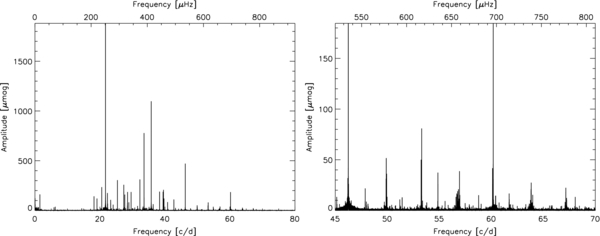
\includegraphics[width=0.8\textwidth]{superstarspectrum.jpg}
    \caption{Figure from \citet{antoci2011excitation}}
    \label{ssspectrum}
\end{figure}

\begin{figure}[htbp]
    \centering
    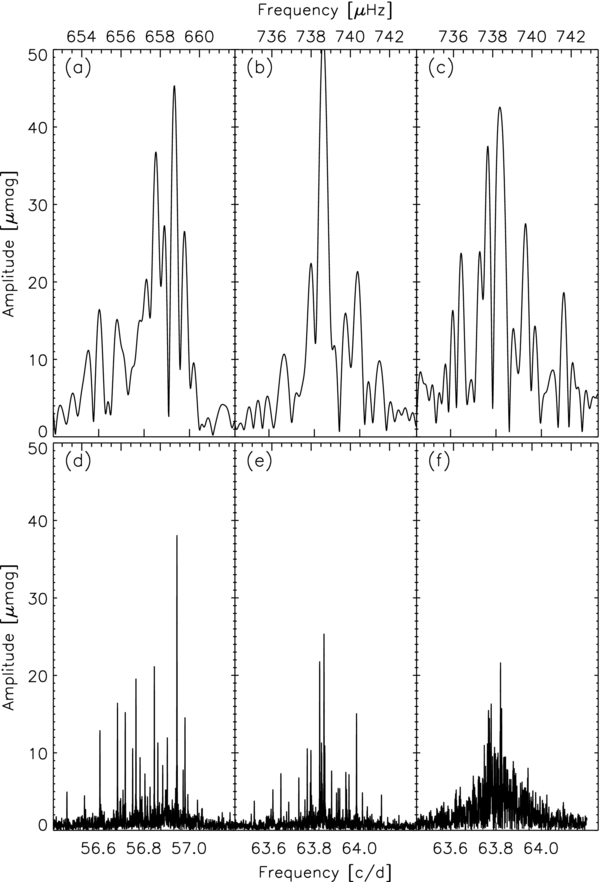
\includegraphics[width=0.5\textwidth]{superstar2.jpg}
    \caption{Figure from \citet{antoci2014role}}
    \label{ss2}
\end{figure}

Besides from the peculiar frequency spectrum, an analysis of the abundances of Superstar classified it as a chemically peculiar Am star. This means that it shows photospheric overabundances in Ba, Y, and Sr and underabundances in Sc and Ca \citep{preston1974chemically}. Particularly of interest are the pulsating AmFM stars, since they do not comply well with predictions from the Kappa mechanism. The theory states that settling of He causes an underabundance in the He II ionization layer, hence the Kappa-mechanism does cannot drive the pulsation sufficiently. \citet{turcotte2000} implemented diffusion of heavy elements into the models to account for only a very tightly constrained instability region. However AmFm are not only observed in this region, but over the entire $\delta$ Sct instability strip \citep{smalley2011superwasp, balona2011kepler}. In that sense, Superstar is interesting not only because of its wide frequency range, but also because those frequencies are even more unusual for a pulsating Am star. Therefore it is of great interest to model this star to gain information on the nature of the pulsations. 
\\
Stellar parameters used 
%Mode identification has not yet provided any reliable results, and further analysis is needed to give information on the nature of the frequencies, and particularly constrain models of the star. 

